\documentclass[11pt]{article}
\usepackage{classTools}

\begin{document}

\psHeader{3}{Wed Oct. 2, 2024 (11:59pm)}

\textbf{Your name: Ethan Veghte}

\textbf{Collaborators: }

\textbf{No. of late days used on previous psets: 2}

\textbf{No. of late days used after including this pset: 5}


The purpose of this problem set is to solidify your understanding of the RAM model (and variants), and the relations between the RAM model, the Word-RAM model, Python programs, and variants. In particular, you will build skills in simulating one computational model by another and in evaluating the runtime of the simulations (both in theory and in practice).

\textit{Note: We STRONGLY recommend typing this problem set (in LaTeX, if possible) -- question 3 will probably be the longest proof we've had you write in the course so far, and unless you have typewriter handwriting, it is much easier for us to grade typed submissions. If we can't read your handwriting, chances are it will lose points.}

\begin{enumerate}
 
    \item (Simulation in practice: RAMs on Python)  
    In the Github repository, we have given you a partially written Python implementation of a universal RAM Model simulator.  Your task is to fill in the missing parts of the code to obtain a complete universal RAM simulator.
     Your simulator should take as input a RAM Program $P$ and an input $x$, and simulate the execution of $P$ on $x$, and return whatever output $P$ produces (if it halts).  The RAM Program $P$ is given as a Python list $[v,C_0,C_1,\ldots,C_{\ell-1}]$, where $v$ is the number of variables used by $P$.  For simplicity, we assume that the variables are named $0,\ldots,v-1$ (rather than having names like ``tmpptr'' and ``insertvalue''), but you can introduce constants to give names to the variables.  The $0$\textsuperscript{th} variable will always be $\inputlen$, the $1$\textsuperscript{st} variable $\outputpointer$, and the $2$\textsuperscript{nd} variable $\outputlen$.  A command $C$ is given in the form of a list of the form $[\cmd]$, $[\cmd,i]$, $[\cmd,i,j]$, or $[\cmd,i,j,k]$, where $\cmd$ is the name of the command and $i,j,k$ are the indices of the variables or line numbers used in the command.  For example,  the command $\var_i = M[\var_j]$ would be represented as $(\READ,i,j)$.  See the Github repository for the precise syntax as well as some RAM programs you can use to test your simulator.

    \item (Empirically evaluating simulation runtimes and explaining them theoretically)  

Consider the following two RAM programs:

\begin{algorithm}[H]
\Input{A single natural number $N$ (as an array of length 1)}
\Output{$13^{2^N+1}$ (as an array of length 1)}
\Variables{$\inputlen, \outputpointer, \outputlen, \counter, \result$}
\setcounter{AlgoLine}{-1}
$\zero = 0$\;
$\one = 1$\;
$\thirteen = 13$\;
$\outputlen = 1$\;
$\outputpointer = 0$\;
$\result = 13$\;
$\counter = M[\zero]$\;
\Indp
 IF $\counter == 0$ GOTO \ref{line:done}\; \label{line:loop}
$\result = \result \times \result$\;
$\counter = \counter - \one$\;
IF $\zero == 0$ GOTO \ref{line:loop}\;
\Indm
$\result = \result \times $\thirteen\; \label{line:done}
$M[\outputpointer]=\result$\;
\end{algorithm}

\begin{algorithm}[H]
\Input{A single natural number $N$ (as an array of length 1)}
\Output{$13^{2^N+1} \bmod 2^{32}$ (as an array of length 1)}
\Variables{$\inputlen, \outputpointer, \outputlen, \counter, \result, \temp, \W$}
\setcounter{AlgoLine}{-1}
$\zero = 0$\;
$\one = 1$\;
$\thirteen = 13$\;
$\outputlen = 1$\;
$\outputpointer = 0$\;
$\result = 13$\;
$\W = 2^{32}$\;
$\counter = M[\zero]$\;
\Indp
IF $\counter == 0$ GOTO \ref{line:done2}\; \label{line:loop2}
$\result = \result \times \result$\;
$\temp = \result / \W$\;
$\temp = \temp \times \W$\;
$\result = \result - \temp$\;
$\counter = \counter - \one$\;
IF $\zero == 0$ GOTO \ref{line:loop2}\;
\Indm
$\result = \result \times \thirteen$\;
\label{line:done2}
$\temp = \result / \W$\;
$\temp = \temp \times \W$\;
$\result = \result - \temp$\;
$M[\outputpointer]=\result$\; 
\end{algorithm}

\begin{enumerate}
    \item Exactly calculate (without asymptotic notation) the RAM-model running times of the above algorithms as a function of $N$.
    Which one is faster? \label{itm:RAMtime}    
    \\\\\textit{
    Lets call the first algorithm $A$ and the second $B$ for the purpose of this question. 
    \begin{enumerate}
        \item Runtime $A$: The first set of operations are initializing, the array, setting constants and creating variables in memory. These are constant time operations, and there are 7 of them. The next set is the looping. This is dependent on how large $N$ is as that is what determines the number of iterations. Within the loop there are a constant set of operations, all of which are arithmetic and thus are constant time. Within the loop it simply does the multiplication and adjusts the counter. Because these are constant time, the exact calculation of the running time is more likely dependent on the number of iterations. To calculate the exact runtime, you sum initialization (7 constant time operations), looping (4 operations: 2 boolean checks, 1 multiplication, 1 decrement) multiplied by iterations ($N$), and outputting (1 final multiplication, and 1 pointer creation). Importantly though, the last time the loop occurs, it has the exit loop line (GOTO) which adds another step of constant time. This results in runtime $ = 7 + N*(4) + 2 + 1 = 10 + N*4$ where N is input natural number. 
        \item Runtime $B$: Algorithm $B$ is very similar to $A$ in structure but it simply has a few more arithmetic operations to do the modulus operation. Similar to $A$ it initializes relevant constants and variables (1 more constant than in $A$). Then, within each loop iteration (number of iteration still dependent on $N$) it performs multiplication, as well as division and then adjusts the counter. This means that an iteration in algorithm $B$ will generally take longer as it requires more constant time operations. To calculate the exact runtime, you sum initialization (8 constant time operations), looping (7 operations: 2 boolean checks, 4 arithmetic, 1 decrement) multiplied by iterations ($N$), and outputting (5 operations: 4 arithmetic and 1 pointer creation). Same as before, there is an additional exit loop operation  This results in runtime $ = 8 + N*(2 + 4 + 1) + 5 + 1 = 14 + N*7$ where N is input natural number. 
    \end{enumerate}
    \\ This means that since exact runtime for $A = 10 + N*4$ and $B = 14 + N*7$ then $A$ should generally run faster than $B$ for equivalent inputs. Especially as for large N
        }
    \item Using your RAM Simulator, run both RAM programs on inputs $N=0,1,2,\ldots,15$ and graph the actual running times (in clock time, not RAM steps).  (We have provided you with some timing and graphing code in the Github repository.) Which one is faster?  \label{itm:realtime} 

    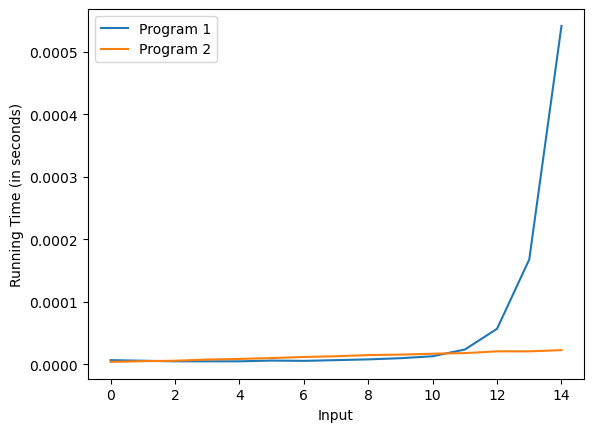
\includegraphics{ps3/running_times.png}

    \textit{We can clearly see that with larger input size, program 2 (B) is faster. From $0 \leq n \leq 10$ program 1 (A) and program 2 (B) have comparable run times. However from $10 < n \leq 15$ and I would suspect beyond 15, program 1 (A) will be significantly slower with respect to physical run time (seconds).
    }
    \item Explain the discrepancies you see between Parts~\ref{itm:RAMtime} and \ref{itm:realtime}.  (Hint: What do we know about the relationship between the RAM and Word-RAM models, and why is it relevant to how efficiently the Python simulation runs?) 

    \textit{
    The reason we see $A$ taking so much longer than $B$ as $N$ increases is because constant time operations just take longer for larger input sizes. This makes sense, because we know computers are more similar to the Word-RAM model thus when there hardware deals with Big-nums it breaks them down to do big-num arithmetic which is more time expensive the larger the number. Even though we counted the arithmetic steps as equivalent no matter the size of the input in ~\ref{itm:Ramtime}, in reality (i.e. how the computer actually computes this operation) this is not true. The discrepancy in time, especially when N is larger, is because in program $B$ \result variable is restricted from growing too big because of the iterative modulus operations throughout the loop. This means the expensive multiplication steps that makes the result number so larger is not able to be that large. In ~\ref{itm:realtime}, however, this does not occur, and \result  can grow to be so large that any operation on it can take a long time. Thus, even though there are fewer operations that occur in program $A$, some operations, despite being considered constant time operations, take longer than others. A computer program can never simulate a RAM model perfectly because at its core a computer is more akin to the Word-RAM model, which values input size in time expenses. This is why we see the timed runtime to take longer on program $A$ than program $B$. 
    }
    \item (optional\footnote{This problem won't make a difference between N, L, R-, and R grades.}) Give a theoretical explanation of the shapes of the runtime curves you see in Part~\ref{itm:realtime}, by providing explicit formulas for the asymptotic runtimes of the two programs (in clock time). You may need to do some research online and/or make guesses about how Python operations are implemented to come up with your estimates. 

\end{enumerate}

\item (Simulating Word-RAM by RAM) For every Word-RAM program $P$, there is a RAM program $P'$ that simulates $P$ in the sense that:
\begin{enumerate}
    \item $P'$ halts on $(w,x)$ iff $P[w]$ halts on $x$, and 
    \item If $P[w]$ crashes, then $P'$ halts with $\outputpointer=\outputlen=0$. (We are using this output setting to indicate \crash, since the RAM model does not have any crashing in its semantics.)
    \item If $P[w](x)$ halts without crashing, then the output of $P'(x,w)$ equals the output of $P[w](x)$.
     Furthermore,   
       $$\Time_{P'}(x) = O\left(\Time_{P[w]}(x)+n+w\right),$$
where $n$ is the length of $x$.

(This was stated without proof in Lecture Notes 8.) 

\end{enumerate}

Your proof should use an {\em implementation-level} description, similar to the proof that RAM programs can be simulated by ones with at most $c$ registers in Lecture 7.  Recall that Word-RAM programs have a finite but changing memory size $S$ and a read-only variable $\wordlen$; you may want to start your simulation by calculating $S$ and $2^{\wordlen}$.  Then think about how each operation of a Word-RAM program $P$ can be simulated in a RAM program $P'$, taking care of any differences between their semantics in the Word-RAM model vs. the RAM model. Don't forget MALLOC!

\textit{
Any program $P$ can be simulated in a RAM program $P'$ because you are able to recognize the differences between the models via O(1) code additions (also one O(n) and one O(w)). In order to prove this we have to address the key differences, which stem out a Word-RAM's capacity to crash and its necessity to deal with changing memory size. The important operations that need to be addressed are arithmetic (+, -, *, /), then read and write, then MALLOC, conditionals, assigning constants, and finally setting outputs. In all of these, since the limitations are input size (which in turn affects memory size because of indexing), the crashing of RAM program must be simulated. Lets first start by calculating $S$  and $2^{\wordlen}$ as is recommended.
\\
Obviously the initial use of memory puts input into M[0]...M[n-1], where n is \inputlen. In order to make a Word-RAM simulation program in a RAM model we then need to simulate the extent of the memory. The memory can only be accessed if it is within an index $< 2^{\wordlen}$. This is because $\wordlen$ tells us the maximum number of bits that can be used, and in binary number system that means the maximum number that can be reached will be $2^{\wordlen}$. To simulate that we need to have a variable two.w that represents that size. Having initialized a set of valuable constants (\zero, \one, \two) along with $s = \inputlen + \zero$, we then have to iterate a multiplication of $\two.w$ and \two, w times:}
\\Set $two.w =one$
\\Set $counter = w$
\\(line 3) IF counter == 0 GOTO 7
\\Set $two.w = two.w * two$
\\Set $counter = counter - one$
\\IF zero == 0 GOTO 3
\\ (line 7) ... 

\textit{
This should successfully create the variable two.w. Now dealing with crashing. Let us use line b as the line at which the crash protocol begins. Should there be a GOTO b command, output.ptr and output.len are 0 and you then jump to last line of code. This section should only be accessed in the event of a crash. The first situation to check is that $S \leq 2^{\wordlen}$. This refers to S as initialized before updating the memory size in any capacity, thus $S = \inputlen$. The steps to check that $S \leq 2^{\wordlen}$ are as follows:
    }
\\\\ set $temp = two.w + \one$
\\ set $temp = temp - S$
\\ IF temp == 0 GOTO b
\\ \textit{Remember that b is the start of the crash protocol. Now that we know memory is not used that is beyond the indexing possibility of $2^w$ we also must check the values within by iterating across all values and checking. This is a slower step that occurs in O(n) time: 
}
\\\\ set counter = 0 
\\ (line 2) set $temp = \inputlen - counter$
\\ IF temp == 0 GOTO line 9
\\ set temp = M[counter]
\\ set $temp = two.w - temp$
\\ set $counter = counter + \one$
\\ IF temp1 == 0 GOTO b
\\ IF zero == 0 GOTO line 2
\\ (line 9) ... 
\\\\\textit{
Now lets represent all the operations of P' in P. 
\\ \textbf{Arithmetic Operations}
\\ The worry with arithmetic operations is that the value exceeds $2^w$. Obviously, / and - in their basic forms used here will not create larger number and thus are not focused on. If they exceed $2^w$ that variable will instead be set to 0. To implement P' we must add that check to any block of code using these operations: 
}
\\set var1 = var2 op var3
\\set $temp = two.w - \one$
\\set $temp = var1 - temp$
\\IF temp == 0 GOTO line 6
\\set var1 = temp (only will be accessed if $var1 > temp$)
\\(line 6)...
\\
\textit{
\\ \textbf{Read and Write}
\\ Read and write are implemented in very similar manners, which fail if the variable called is outside the size of our memory store S. In the case that it is called something outside of S, there is not effect. The simulation then of $var1 = M[var2]$ looks like:
}
\\ set temp = s - var2 
\\ IF temp == 0 GOTO line 4
\\ var1 = M[var2] 
\\ (line 4) ... 
\\
\textit{Write is the same logic but for the opposite direction in which you write some value var1 in some memory location var2. But the check of memory capacity still stands. \\
\\ \textbf{MALLOC}
\\ In the situation in which MALLOC is called the concern is that the next allocated piece of memory goes beyond the capacity that memory can be accessed. To do this we use S as the changing size of memory. If we have room to increment we increment, otherwise we send to crash protocol:
}
\\ set $temp = two.w - S$
\\ IF temp == 0 GOTO b
\\ set $S = S + \one$
\\
\\ 
\textit{
\textbf{Conditionals}
\\ Conditionals are easy, because nothing changes, but the line number that is referenced after adding more code blocks to properly simulated P'. So if it previously referenced line 4, it might now need to recognize line 10. Lets call that change from line z to line z', so
\\IF \dots GOTO z $\Rightarrow$ IF \dots GOTO z'
\\\\
\textbf{Constants}
\\This is for assignments that look like var = c. The check for this scenario is to just ensure that constant $c < 2^w$. If this fails, the program should go to crash protocol. The simulation looks like: }
\\set temp = c
\\set temp = temp - S
\\IF temp == 0 GOTO b (b is crash protocol)
\\set var = c \\
\textit{
\\ \textbf{Setting output}
\\ The final operation/command that is to be recognized is setting an output. Remember that the output will be (M[0], \dots M[min(output.ptr + output.len -1], S-1). This is easy to do, and lets say f, for final, is the final line of code.
}
\\ 
\\set temp = output.ptr + output.len
\\set temp.1 = temp.0 - S
\\IF temp.1 == 0 GOTO line f
\\set output.len = S - output.ptr
\\set output.len = output.len - 1
\\IF zero == 0 GOTO f

\textit{
\\\\ This concludes the use cases of our simulation, but now we just have to ensure that the few statements from the beginning are maintained. Since RAM program P' simulates Word-RAM P in the methods we described above we know it does so in a few important ways. First, in all of the adjustments, they are done in O(1), non-looping lines of code, except for creating variable two.w which is done in O(w), and also checking that all the values are less than $2^w$ which is done in O(n) where n is input size. With this we we know we do not sacrifice the output values of P so if $P[w](x)$ halts without crashing, then the output of $P'(x,w)$ equals the output of $P[w](x)$. Also, if P' halts on $(w,x)$ iff P[w] halts on x. We also know that we properly dealt with the cases in which it crashes so that in these cases output.len and output.ptr are set to 0. This validates the statement f $P[w]$ crashes, then $P'$ halts with $\outputpointer=\outputlen=0$. Finally, as we talked about above witht the adjustments in runtime, we know that the only changes are in O(1), except for two cases where they are O(n) and O(w) thus $$\Time_{P'}(x) = O\left(\Time_{P[w]}(x)+n+w\right),$$
where $n$ is the length of $x$. 
}

\item (reflection) Discuss the value (or lack thereof) that you think computational models, and the RAM and Word-RAM models in particular, have for computer science.  All opinions are valid, as long as they show serious thought and are backed by specific justifications.

\textit{Note: As with the previous psets, you may include your answer in your PDF submission, but the answer should ultimately go into a separate Gradescope submission form.}


\textit{
I think there is some value in understanding the Word-RAM model as it helps us understand the limits to the physical hardware that computers more realistically represent. I struggle to see the relevance of learning the RAM model. I see that it adds context to the Word-RAM model in that you are able to recognize their differences, but I find it difficult to see why we almost spent more time on it then the Word-RAM model. I think it would have been just as useful to introduce the Word-RAM model, and offer the RAM as an alternative with less restrictions. Instead, we introduced RAM first, but were then told "oh that is actually unrealistic computers are more like the Word-RAM model...". Despite this criticism, I do think this PSET helped me a lot in wrapping my head around these concepts, as I was quite confused coming out of lecture.
}
\item Once you're done with this problem set, please fill out \href{https://forms.gle/TG8cG4LWN3S4T6za6}{this survey} so that we can gather students' thoughts on the problem set, and the class in general. It's not required, but we really appreciate all responses!

\end{enumerate}


\end{document}
